% Instructions to modify this document:
% * Remember to ALWAYS execute a git pull BEFORE any commit you make
% * Use the \ToDo{...} command to remark tasks which still need to be done
% * Use the \input{file.tex} command to split the document into several parts
% * Do not change the current LaTeX coding style to yours

% To convert .dia diagrams into PDF:
% 1) Create the diagram with dia (or any other tool)
% 2) Export it as .eps
% 3) use epstopdf to convert to PDF


\documentclass[a4paper,12pt]{article}

\usepackage[utf8]{inputenc}
\usepackage{amsmath,graphicx}
\usepackage{bm}
\usepackage{amssymb}
\usepackage{algorithm}
\usepackage{algpseudocode}
\usepackage{subfigure}
\usepackage{ifpdf}
\usepackage{url}
\usepackage{color}
\usepackage[hidelinks]{hyperref}
\usepackage{comment}
\usepackage{float} % To put figures in their exact place with \begin{figure}[H]

% Definitions and commands
\def \np{\vskip 0.25 cm}
\def \ap{\vskip 0.15 cm}

\newcommand{\ToDo}[1]{\textcolor{magenta}{\textbf{[ToDo]} \textbf{#1}}}


\begin{document}


\begin{titlepage}

\begin{center}
\vspace*{-1in}

%Universitat Oberta de Catalunya\\
\vspace*{0.6in}
\begin{Large}
\textbf{The IPOL Demo System} \\
\end{Large}
\vspace*{0.6in}
\rule{80mm}{0.1mm}\\
\vspace*{0.1in}
\end{center}

\end{titlepage}

%\maketitle
\newpage

\tableofcontents
\newpage
\listoffigures
\newpage


% The Blobs module
\section{The Blobs module}


\subsection{Introduction}
\label{sec:blobs_introduction}
Necessarily, management of this part is very important. Nowadays, each demo owns images.
Even if they are not heavy (minus 1 MB),
when there are fifty different demos on system and each demo is downloaded using
\textbf{GitHub\footnote{\cite{GitHub}}} then the compilation of system takes too much time.
Knowing that each
demo details a mathematic theory with complex calculations and several demos use
same images, it will be preferable to create a system to manage theses images. \\
\setlength{\parindent}{0cm}

Before specifing this abstract system, it must be known with precision how the actual system
works.\\
\setlength{\parindent}{0cm}

According to the provided UML (\ref{img:IPOL_diagram_class}), one class "image" implements
functions changing image characteristics. To do it, it uses \textbf{PIL\footnote{\cite{PIL}}}.
Images have two formats: thumbnail and an input image. Thumbnail allows the user visualize
and select an input image on client side. Input image is which use to apply algorithm on it,
algorithm specific to the demo. This part is made in the implementation of demo.
Moreover, configuration file allows to customize the default input files.
The images are stored in a directory ("/input"). When using client side of the demo to test
it, new images are generated and stored in a temporary directory in ("/tmp").\\
\setlength{\parindent}{0cm}

\begin{figure}[H]
  \centering
  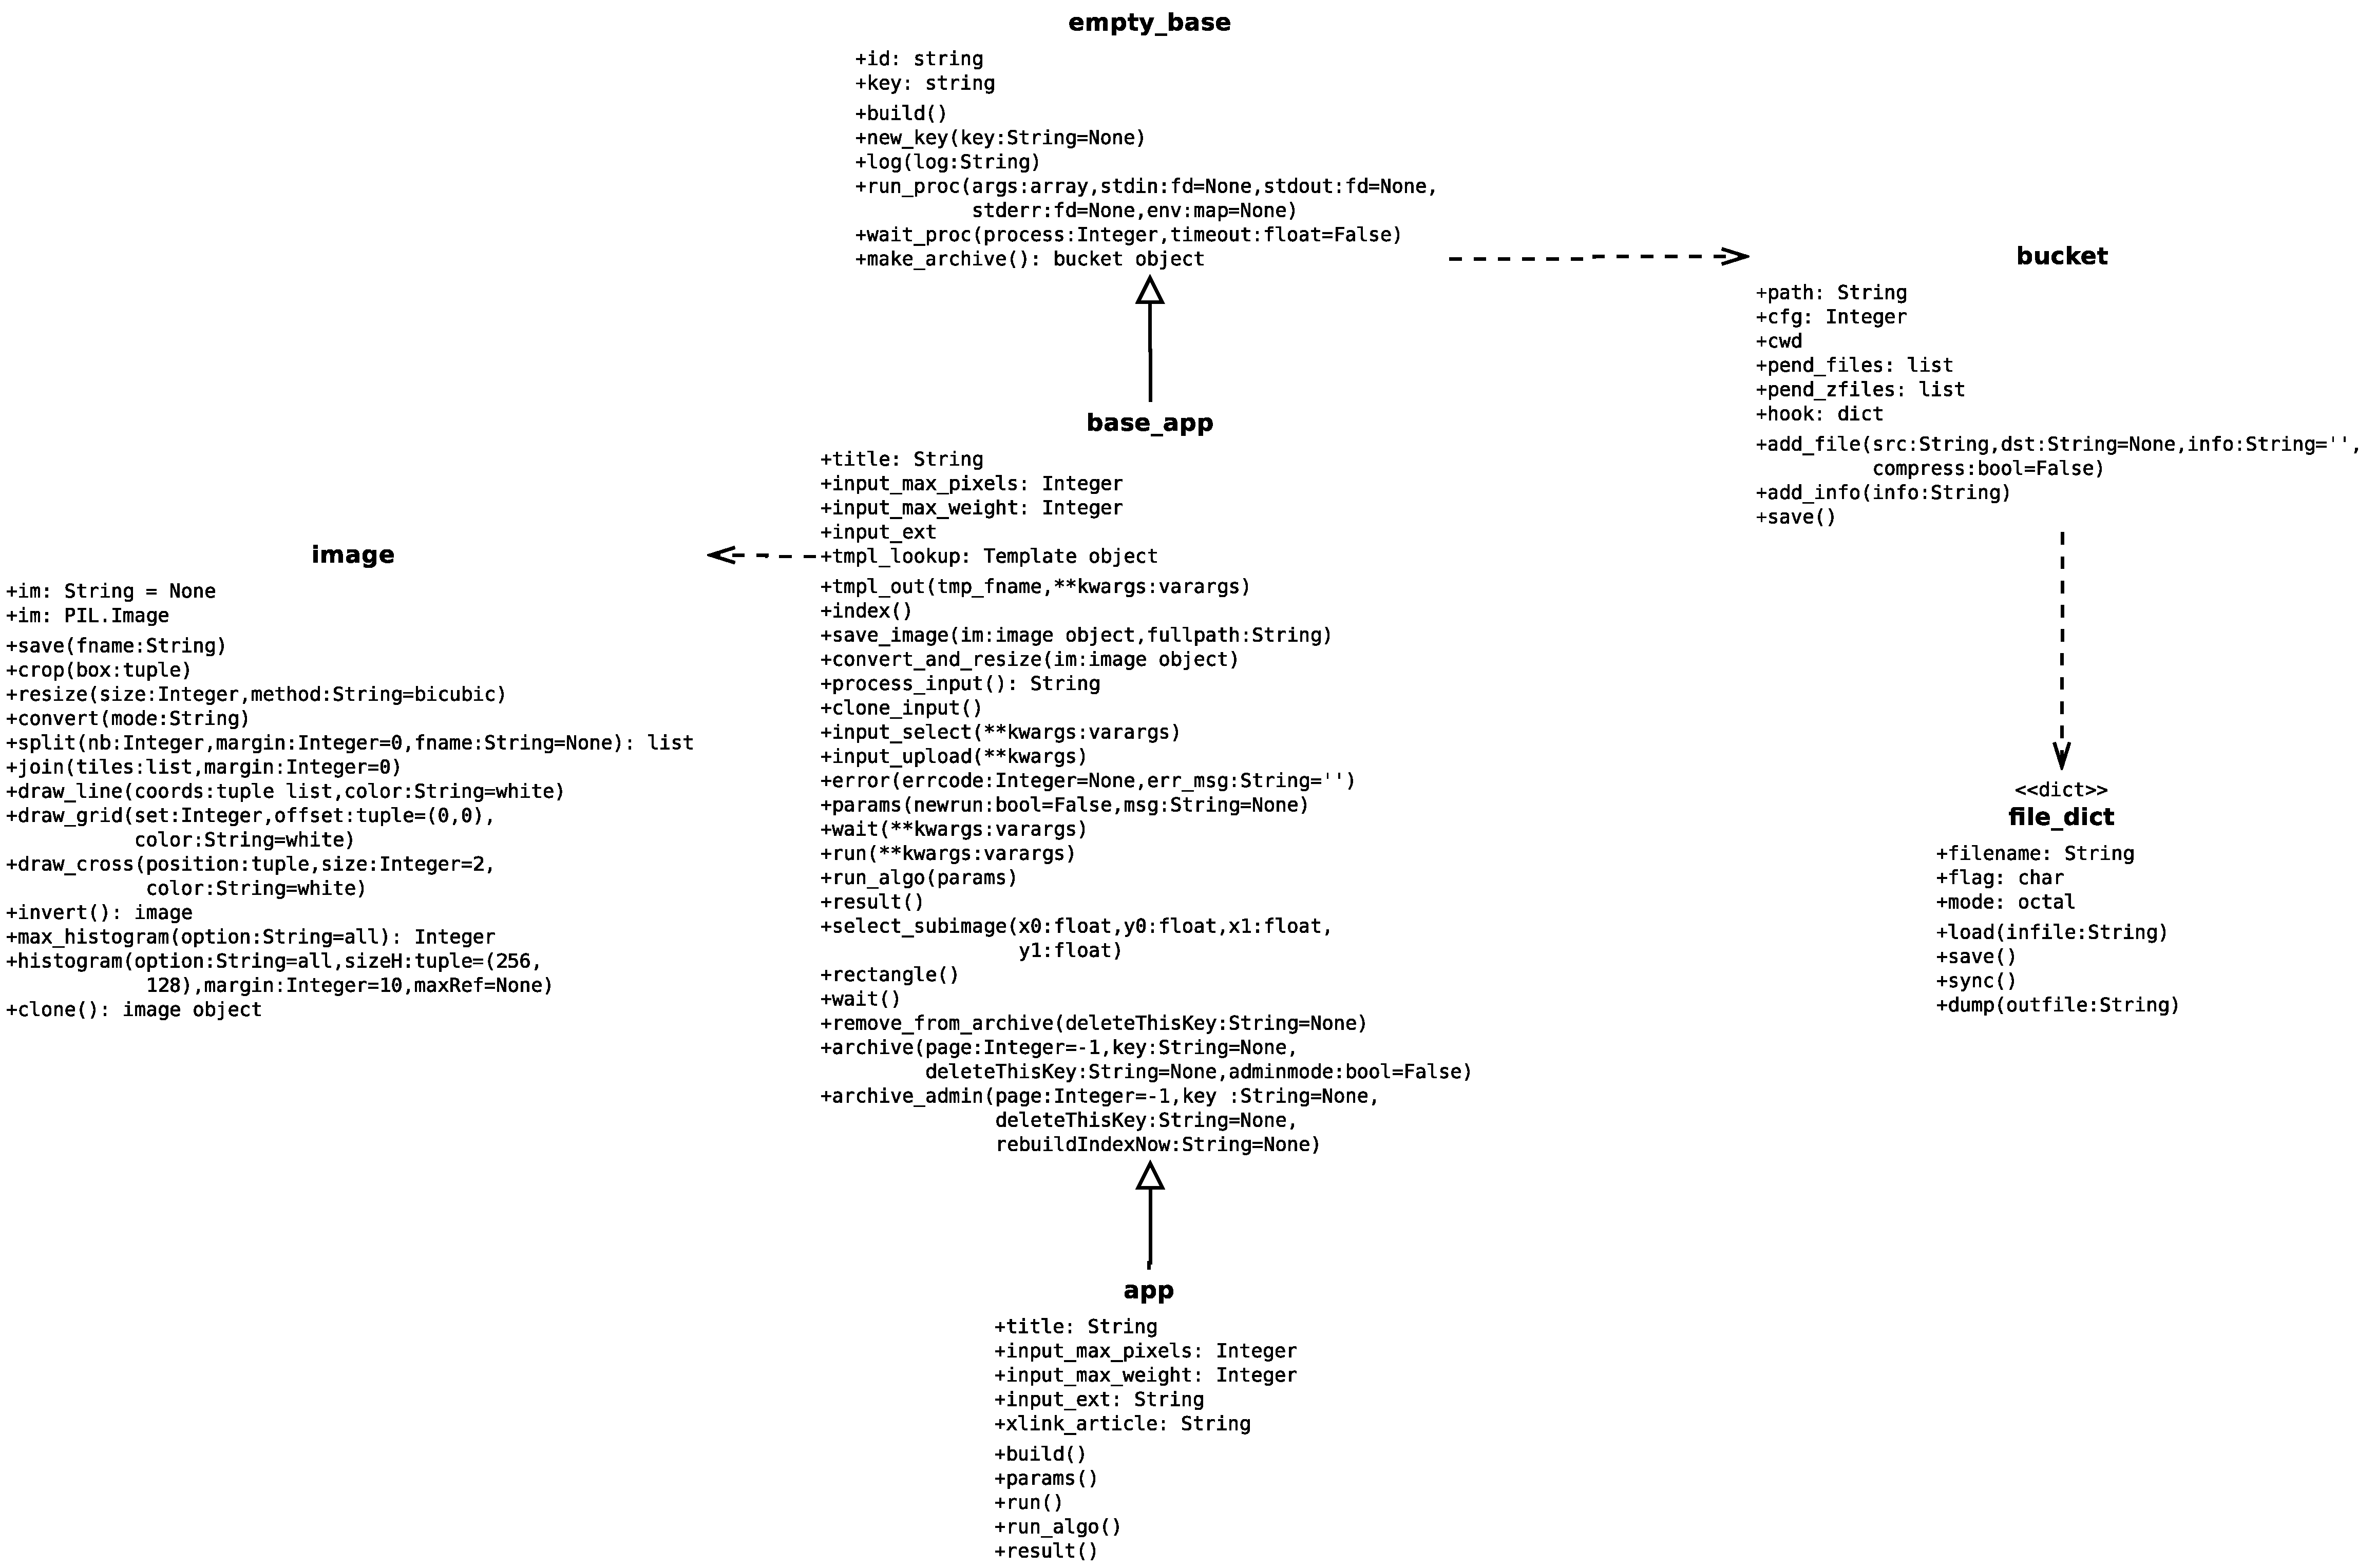
\includegraphics[width=20.0cm, angle=90]{blobs/images/IPOL_diagram_class.pdf}
  \caption{UML diagram class of current system.}
  \label{img:IPOL_diagram_class}
\end{figure}

To conclude this part, images are result of demo and the management of these is important
for the project.

\subsection{Demo}
During introduction, demo system will claim like "God Object". It is excessive term in
order to represent the system with a metaphor. It is just a complex object.
In this section, it will detail functionalities to clarify objective thereof and
look how it is possible to improve it.\\
\setlength{\parindent}{0cm}

Firstly, this object introduce here (\ref{img:IPOL_diagram_class}), has many ways to
interact with user. It implements all features of project. For example, it manages
interaction with client side. To do so, it is a part of webserver developed in
\textbf{CherryPy\footnote{\cite{CherryPy}}}.
Communication between the client and the server is done using an
\textbf{HTTP\footnote{\cite{HTTP}}}. Indeed, when users call a functionality,
this object allows to search the expected result. For example, when users call an algorithm,
it runs the corresponding binary in "bin/" file, manage images archiving the result
and call the HTTP response using the \textbf{Mako Template Library\footnote{\cite{Mako}}}.
Knowing these possibilities, it is very difficult to add new functionalities to this object.
\\
\setlength{\parindent}{0cm}

To conclude this part, the demo is a powerful object but to go further, it needs to create
separate module which communicate with the core system.

\subsection{Solution}
\setlength{\parindent}{1cm}
\hspace{1cm}

Since the problematic have been detailled, it will be necessary to solve it. In this part,
it will present to you \textbf{MVC pattern}, \textbf{Factory pattern}, \textbf{Database}.

\subsubsection{MVC pattern}
\setlength{\parindent}{1cm}
\hspace{1cm}

MVC, alias Model-View-Controller, is architectural pattern used in interface implementation.
It consists of create three separates parts. The model manage database and it is observable
object. The aim of view is to update data from model and to notify event, which by user,
to controler. The controler receive notification from view and update the model.
\setlength{\parindent}{0cm}
In our case, the model will be protocol used to interact with database of images.
The view is client side which look by users using them browser.
It will be updates in the control of the web page on client side.
The controler will be the code used to manage new module implementing functionalities.



\begin{figure}[H]
  \centering
  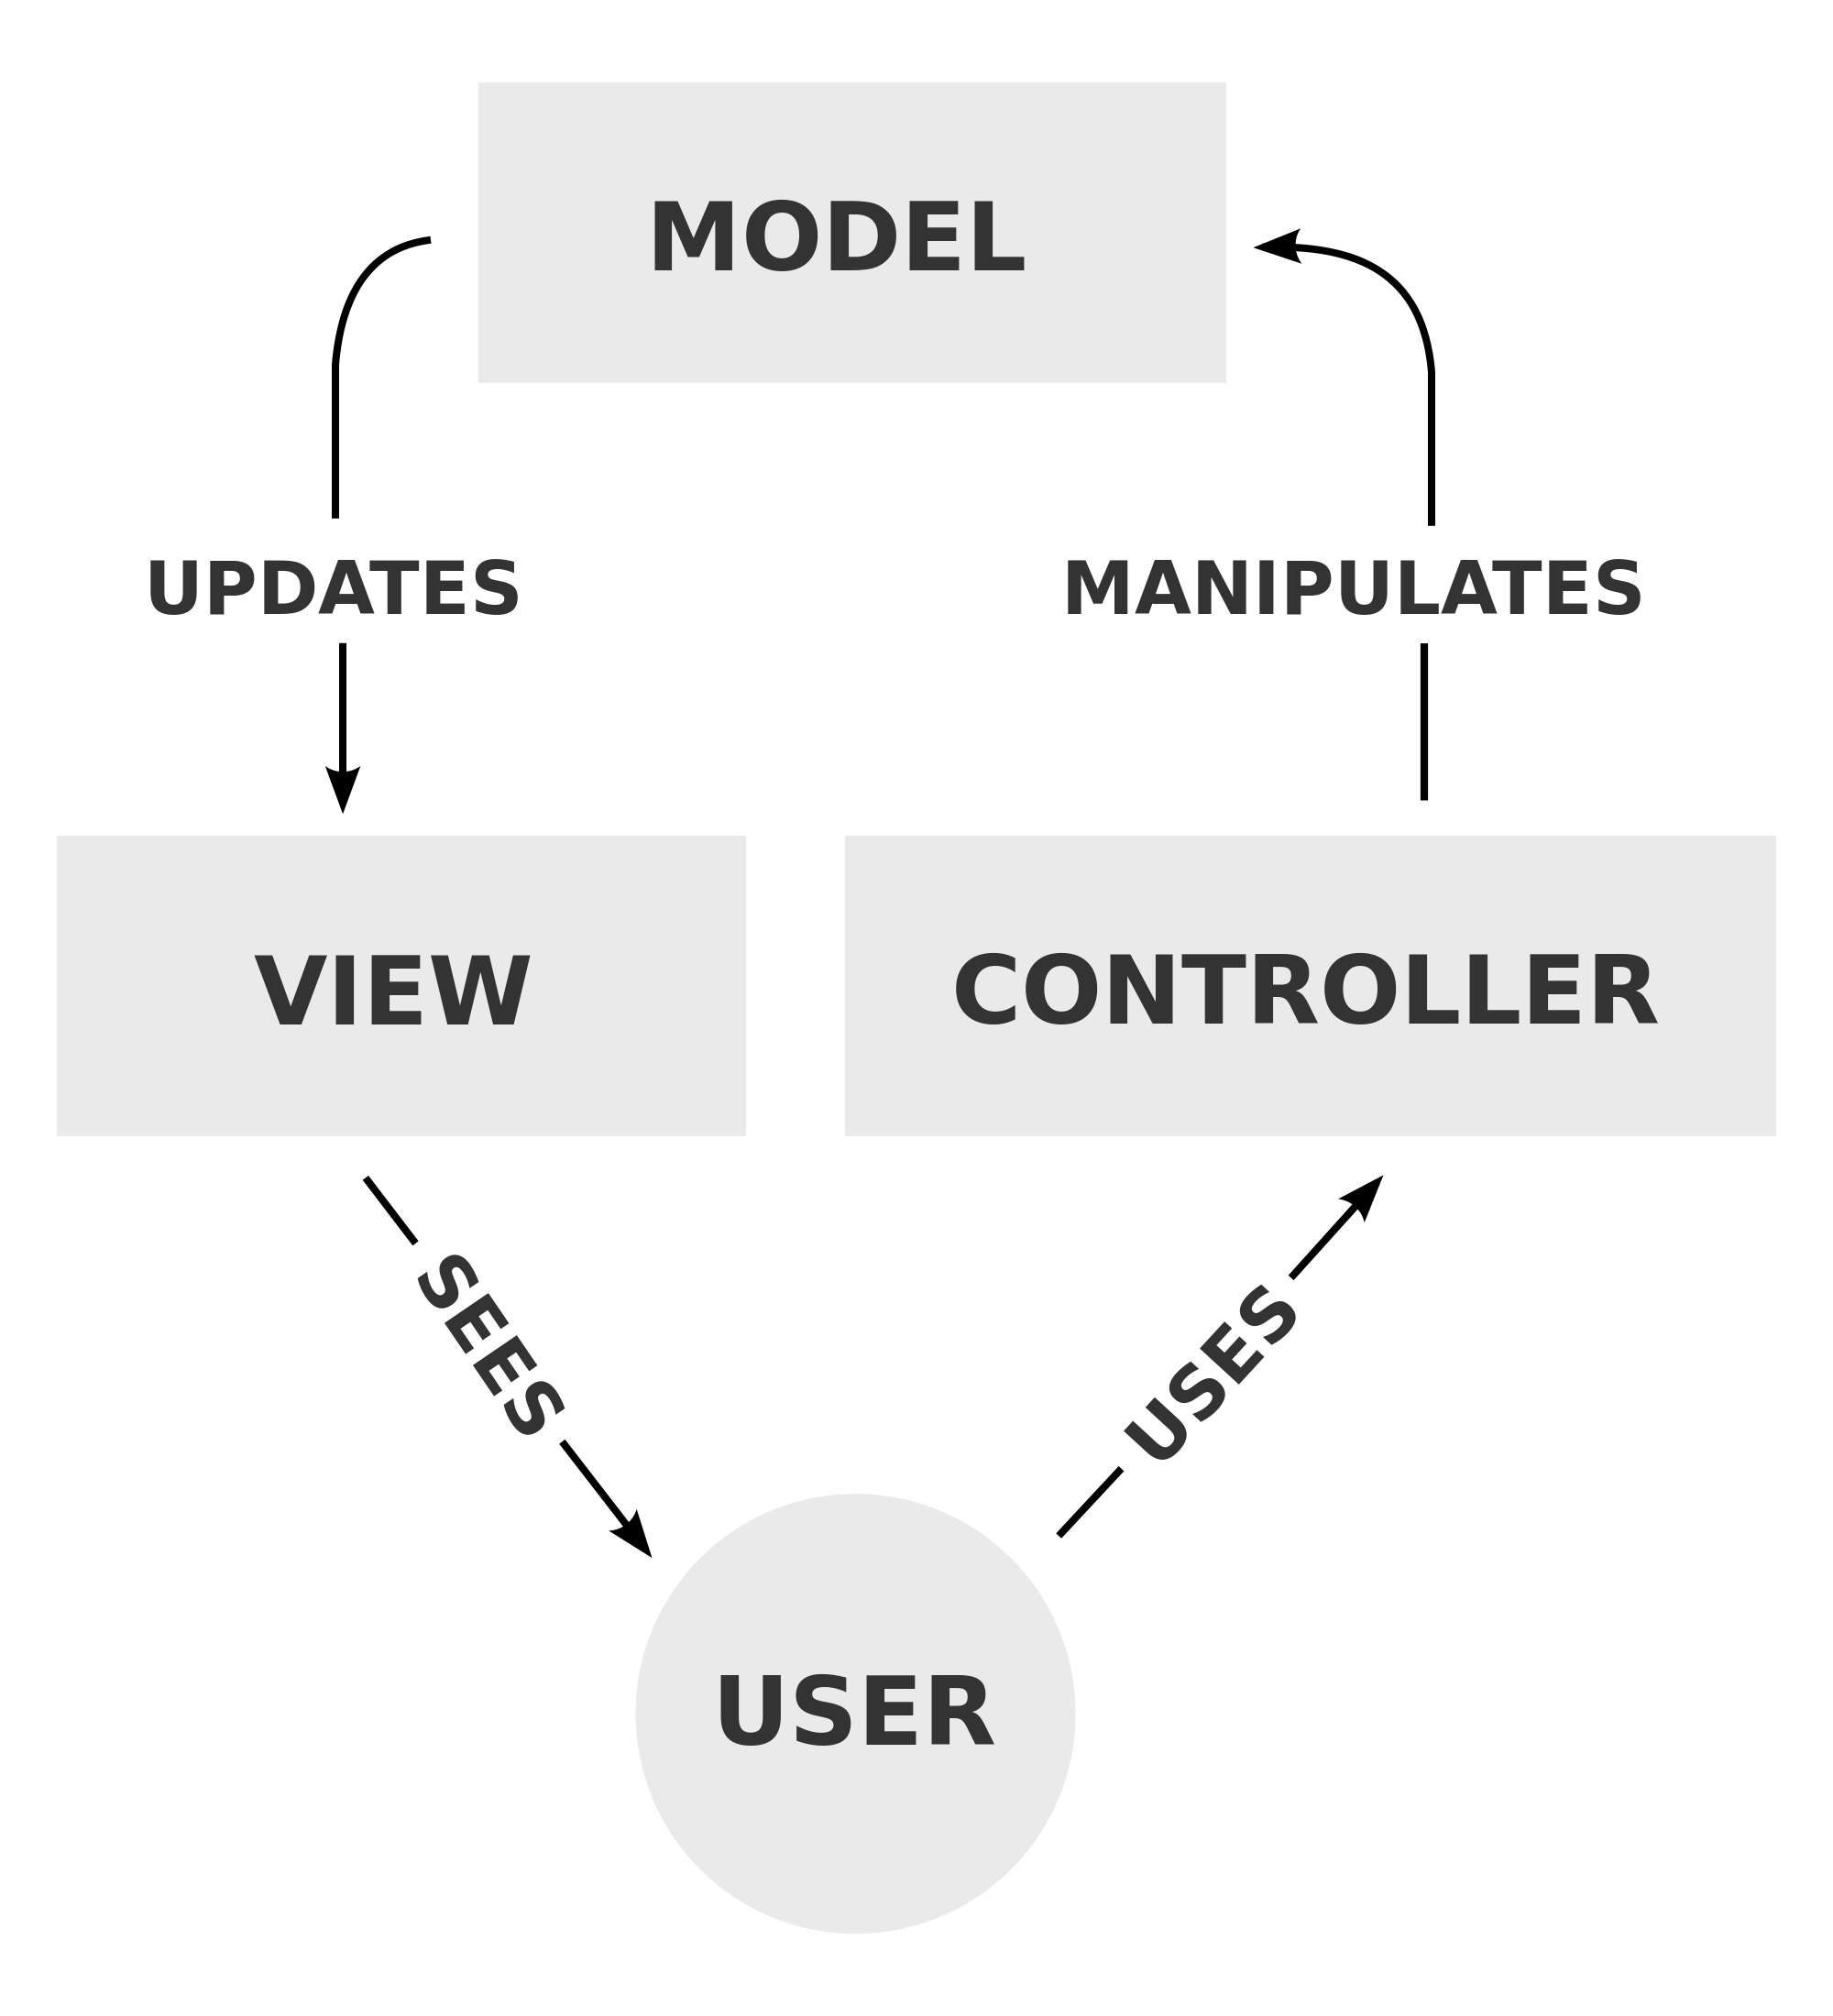
\includegraphics[width=3.5in]{blobs/images/MVC-Process}
  \caption{The MVC pattern}
  \label{img:MVC-Process}
\end{figure}

\subsubsection{Factory pattern}
\setlength{\parindent}{1cm}
\hspace{1cm}
\ToDo{[Miguel] The factory pattern is not used in the new system, since finally
backwards compatibility needs not to be ensure. 
This section should be removed.}

Factory is a \textbf{design pattern\footnote{\cite{GoF}}} allowing to create other objects.
In order to explain the Factory pattern, it must know what is an inheritance.
In inheritance based on object-oriented
programming, it is possible to create an interface (or abstract class) which two different
classes inherit. The most famous example should be the interface Animal which is defined that
Animal could have and it must have to be animal. Dog and Cat are two different classes
inheriting each one from Animal class.
Factory, in this case, could be Farm class. In function to the type of animal which you want
to create (ex: 1 for Cat and 2 for Dog), the Farm will instantiated one of two ways like
Animal class. To do that, it can use implicit or specific cast, it depends of language of
programming.
\bigbreak
\setlength{\parindent}{0cm}
In our case, it will have two versions of demos. The first one like it is nowadays, and the
second one which will be interact with new module. The aim factory is to create just one
object instantiating one of two ways. Consequently, it will be easier to make it work both
version on the same system.

\begin{figure}[H]
  \centering
  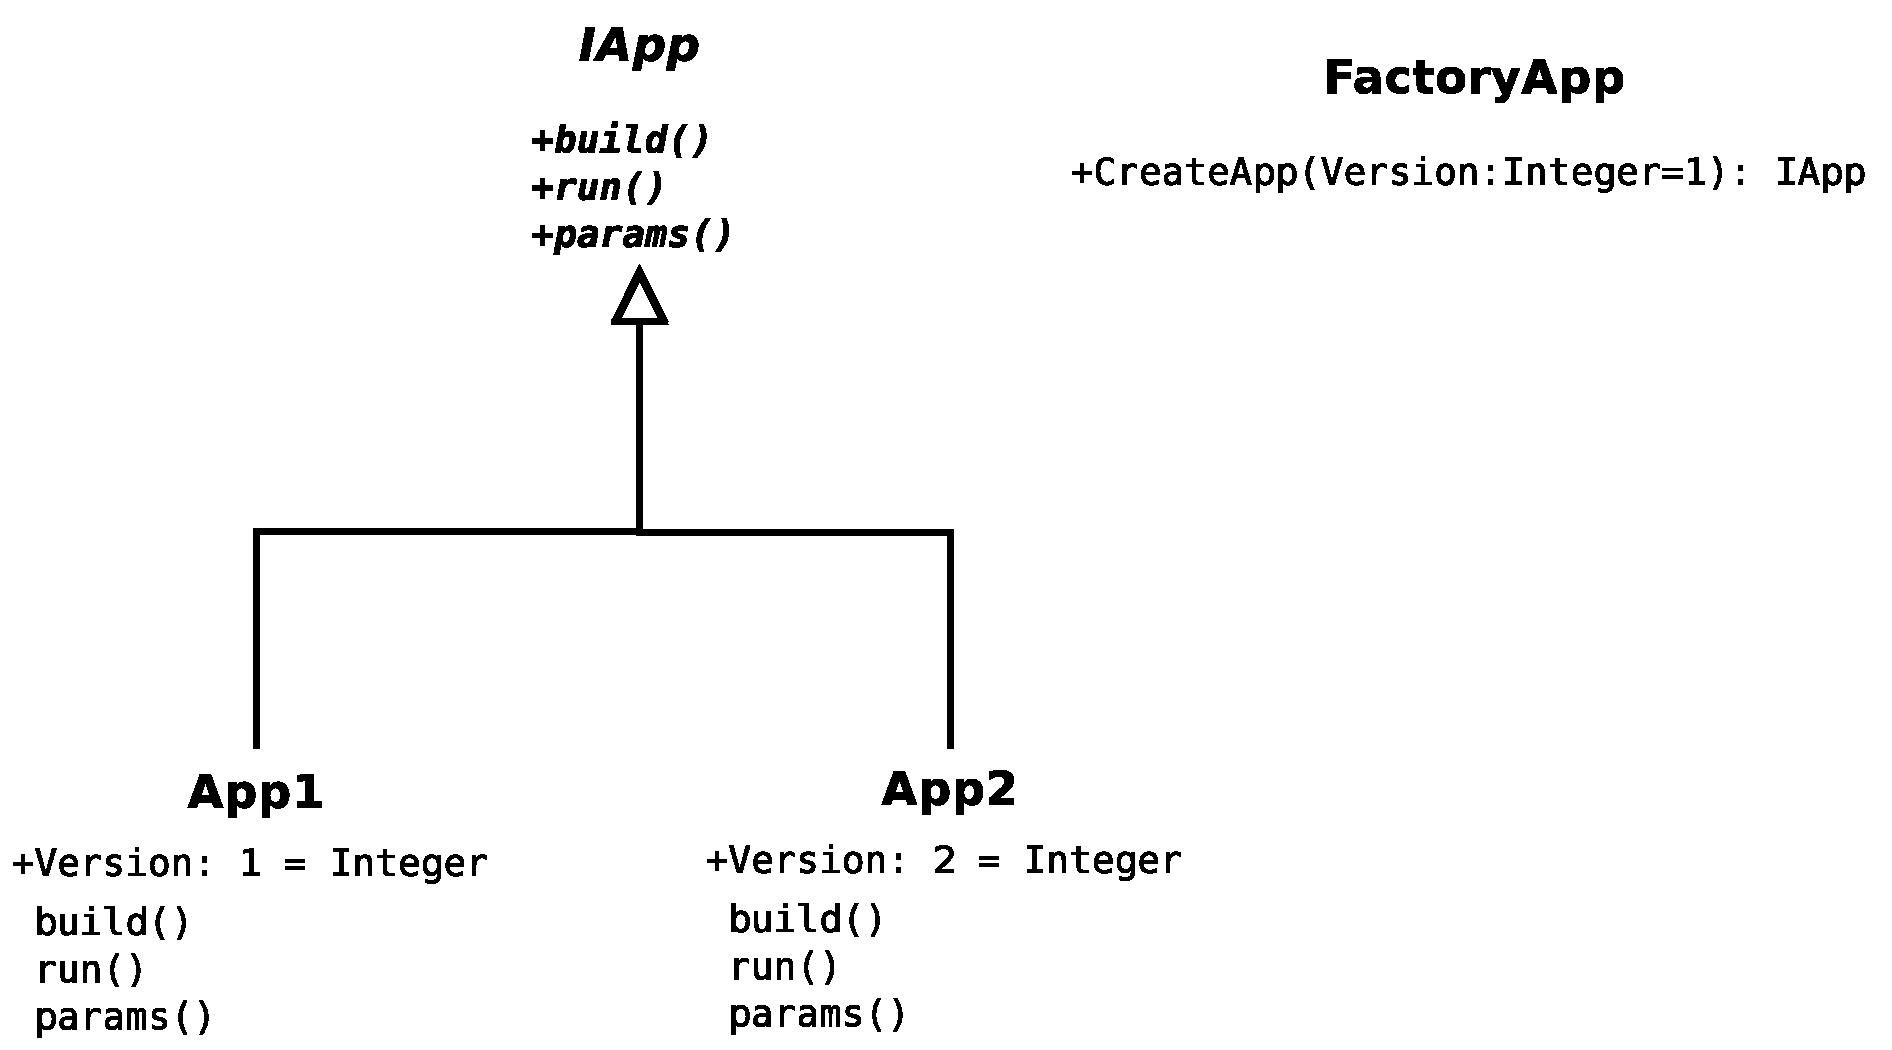
\includegraphics[width=5in]{blobs/images/Example_Factory_Pattern}
  \caption{An example of Factory pattern}
  \label{img:Example_Factory_Pattern}
\end{figure}

\subsubsection{Database}

To solve the problem of images management, it will have a database. It will use a
back-end and will be created with \textbf{SQLite\footnote{\cite{SQLite}}}.
It will have different tables
containing all informations about images. In this way, it will be more easier to
add functionalities and access to images from anything demo. According MVC pattern,
this database will be very useful.\\

\begin{figure}[H]
  \centering
  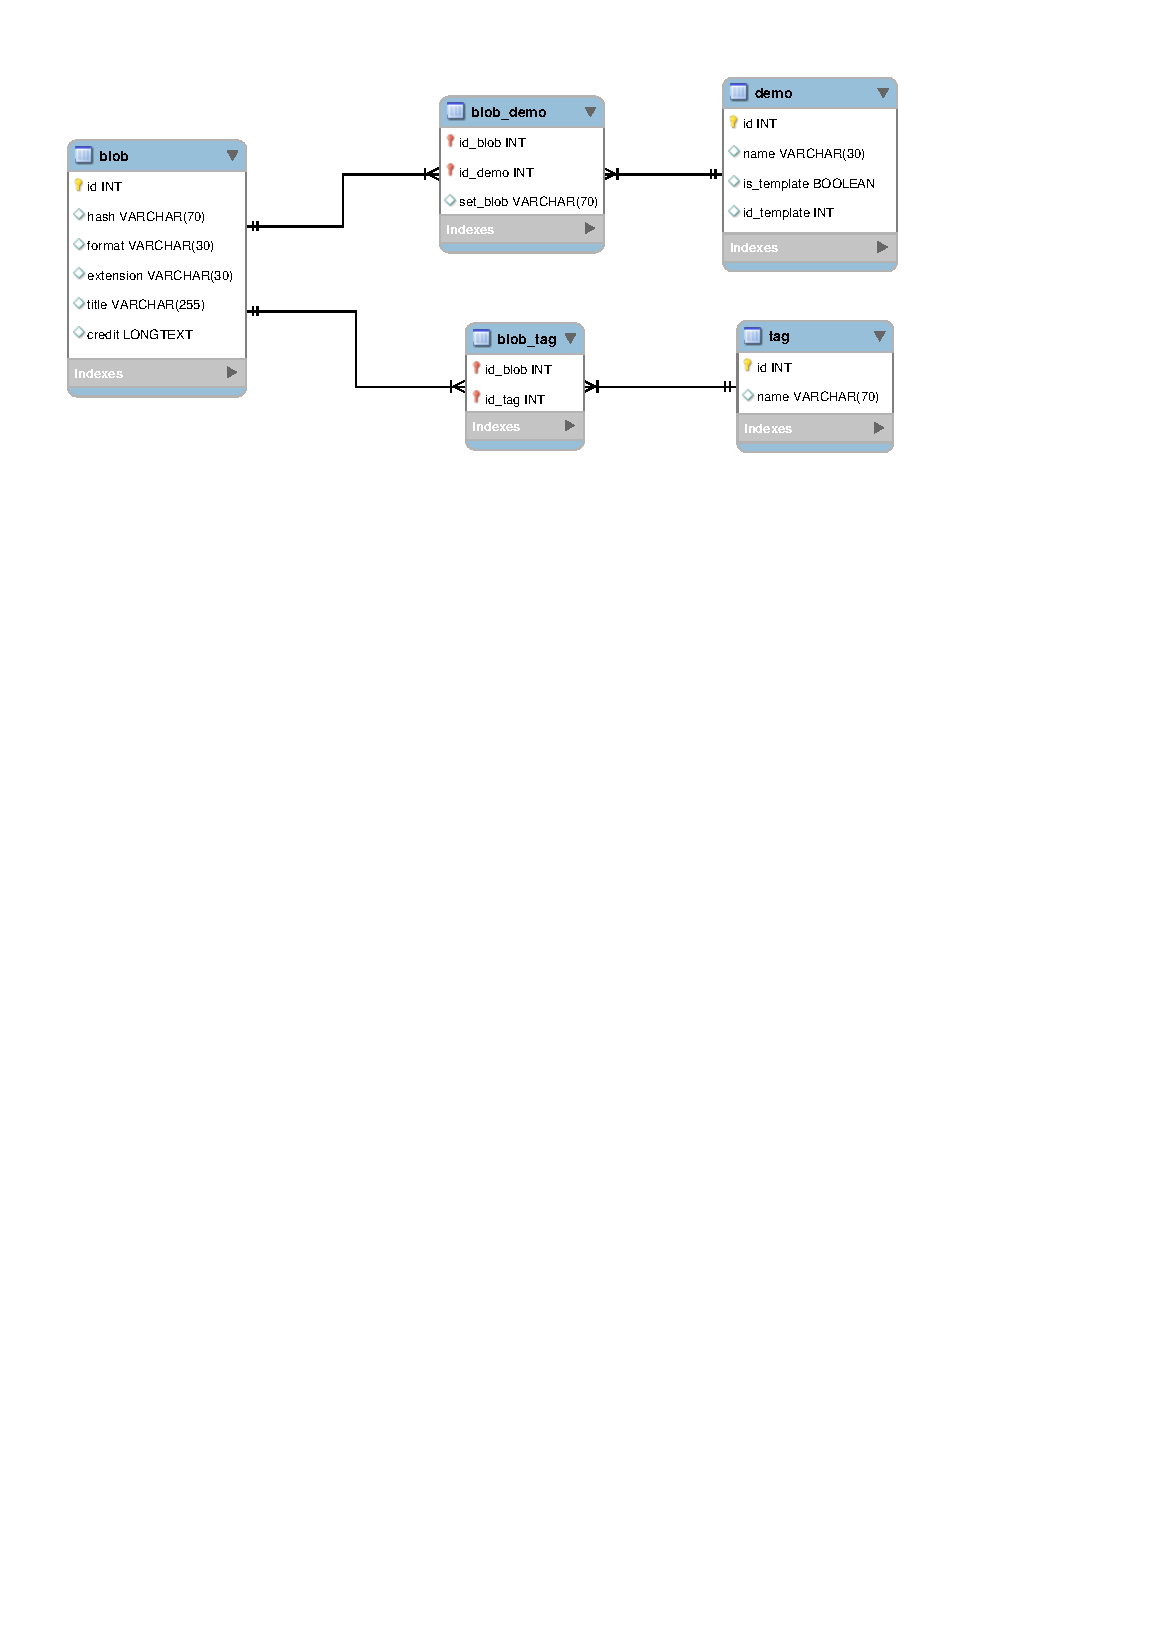
\includegraphics[width=5in]{blobs/images/images_bdd}
  \caption{Database schema for the Blobs module. \ToDo{The image contains a large black at the end and fills out all the page! Fix this.}}
  %\footnotesize
  %\caption*{Realized with MySQL Workbench}
  \label{img:images_bdd}
\end{figure}

\subsection{Remarks}
\subsubsection{Concurrent accesses}
\setlength{\parindent}{1cm}
\hspace{1cm}
The library used to insert, select or update database is
\textbf{SQLite\footnote{\cite{SQLite}}}. This thereof manages, internally,
the concurrent access to database. Indeed, when two people want to
access to the database : the first one will do his request while
the other will be locked by mutex. This principle is also used by transactions
(BEGIN or END/COMMIT).
Therefore, at the beginning of development, it was thought only need a
connection to the database.\\
The problem of the concurrent accesses has been raised during errors occured.
Indeed, when errors occured, the program throws exception and call "roll back"
database's function. Imagine that some people try access to the same data and to
modify it, but some successed it and some failed. The problem of using a only
connection is how to know what changes have been taken into account knowing
that for certain, the database rolled back.\\
Therefore for each request requiring the database,
a new instance (new connection) is used. Thus, the problems
of "roll back" are avoided. Nevertheless, it would be preferable to use a decorator
to avoid the redundance of the code.

\subsubsection{Consistency check}

The consistency check in database management system (DBMS) is the fact
to verify the consistency between the information present on hard disk and
those present on database.\\
There are two ways to do this: running database consistency check manually and
automatically. The program uses consistency check manually in order to
having the control on the error occuring.\\
That is why, when the program uses the action database (SELECT, DELETE, UPDATE),
each information is checked. If errors occurs, an database's exception is caught
and custom exception is throwed to called function.
The consistency check manually is also used because the design databse
has some constraints like: "DELETE CASCADE" and "UPDATE RESTRICT".

\subsubsection{Use case: Web service}
\ToDo{Some of the information here is inconsistent with the actual API implemented in the module. Fix it.}
\ToDo{Think of a better way to describe the webservice API, rather than a table.}

\begin{flushleft}
\begin{longtable}
                   {|C{\dimexpr 0.40\linewidth-2\tabcolsep}
                     ||
                    L{\dimexpr 0.6\linewidth-2\tabcolsep}|}
% {|C{\dimexpr 0.30\linewidth-2\tabcolsep}||
%                     C{\dimexpr 0.20\linewidth-2\tabcolsep}|
%                     C{\dimexpr 0.18\linewidth-2\tabcolsep}|
%                     C{\dimexpr 0.32\linewidth-2\tabcolsep}|}
%   \hline
%   {\bf Function Name} & {\bf Description} & {\bf Param.} & {\bf Return} \tabularnewline
  \hline
  {add\_blob\_ws}
                  & add blob to database \\
                  & {demo\_id path tag ext the\_set title credit} \\
                  & {\{  return:OK or KO, the\_hash: ...  \}} \\
  \hline
  {add\_demo\_ws}
                  & add demo to database \\
                  & {name is\_template template }\\
                  & { \{ return:OK or KO \} }\\
  \hline
  {add\_tag\-\_to\_blob\_ws}
                  & add tag to database \\
                  & { blob\_id tag }\\
                  & { \{ return:OK or KO \} }\\
  \hline
  {delete\_blob\_ws}
                  & delete blob from id demo and id blob \\
                  & {demo\_id blob\_id} \\
                  & { \{ return:OK or KO, delete: (hash, extension) \}} \\
  \hline
  {demos\_ws}
                  & list demos present  in database \\
%                   & { }\\
                  & {\{ return:OK or KO,
                        list\_demos: \{id:name, id\_template, template \} \}} \\
  \hline
  {get\_blob\_ws}
                  & return blob information from id \\
                  & {blob\_id }\\
                  &  {\{ return:OK or KO,
                        \{id, hash,  extension, credit \} \} }\\
  \hline
  {get\_blobs\-\_from\-\_template\_ws}
                  & list blobs from name template \\
                  & {template} \\
                  & { \{ return:OK or KO,
                        blobs: \{id, hash,  extension, format \} \} }\\
  \hline
  {get\_blobs\-\_of\-\_demo\-\_by\_name\_ws}
                  & list blobs from demo name \\
                  & {demo\_name }\\
                  & { \{ return:OK or KO,
                        blobs: \{id, hash,  extension, format \},
                        use\_template: \{id: name, is\_template, id\_template\}\} }\\
  \hline
  {get\_blobs\-\_of\-\_demo\-\_ws}
                  & list blobs from demo id \\
                  & {demo }\\
                  & { \{ return:OK or KO,
                        blobs: \{id, hash,  extension, format \},
                        use\_template: \{id: name, is\_template, id\_template\}\}}\\
  \hline
  {get\_tags\_ws}
                  & return list tags from blob id \\
                  & {blob\_id} \\
                  & { \{ \{id: name\} \} }\\
  \hline
  {get\_tem\-plate\-\_demo\-\_ws} 
                  & return list demos templated \\
                  &  {}\\
                  &  {\{ return:OK or KO, list\_template: \{id: name\} \}} \\
  \hline
  {op\_remove\-\_demo\_ws}
                  & remove demo from id demo  \\
                  & {demo\_id }\\
                  & { \{ return:OK or KO \} }\\
  \hline
  {remove\_tag\-\_from\-\_blob\-\_ws}
                  & remove tag for a blob from id tag and id blob  \\
                  & { id tag\_id blob\_id }\\
                  & { \{ return:OK or KO \} }\\
  \hline
  {set\-\_template\-\_ws}
                  & change the current template used by a demo \\
                  & { demo\_id id name }\\
                  & { \{ return:OK or KO \} }\\
  \hline
\end{longtable}
\end{flushleft}




% The Archive module
\section{The Archive module}
\label{sec:archive}


\subsection{Introduction}
\label{sec:archive_introduction}

%\paragraph{Introduction} \hspace{0pt} \\
The archive module is a standalone application destined to communicate with other modules using webservices. It is designed to implement a stable, simple, and scalable system for archiving all experiments done with IPOL.

\paragraph{Technologies used} \hspace{0pt} \\
The archive module, written in Python, is using fastAPI for webservices, Python Image Library for thumbnails creations, and the python-magic library available on pip (not to be mistaken with python-magic5 which is the one available on the Ubuntu repositories). The module communicates using JSON, both in input and output. The database engine used is SQLite.

\subsection{Architecture}

\paragraph{Module composition} \hspace{0pt} \\
The module is composed of very few files, the code itself in ``archive.py'', a ``router.py'', and a database.

\paragraph{Module architecture} \hspace{0pt} \\
The module is composed of a class, 'Archive', encapsulating the data needed to function. The services offered by the module are all methods of this class. FastAPI will expose all archive http endpoints to make them available and take incoming requests. \\
Upon starting the core module, it will mount archive's router where all endpoints are defined. If they don't exist, both the database and the directories needed for the storage of blobs, logs, the database and thumbnails will be created in their corresponding locations specified in the ``config.py'' file, provided that the user launching the module has the necessary rights. Otherwise, the module will not start. These directories are indicated in the ``config.py'' file, if they are missing from it, the module will not start. \\
The services all connect to each database in a thread-safe way, instanciating its own connection when called, commiting when done if there are modifications, or rollbacking individual queries, if there is an error, and closing the connection. \\
There is a logger initialised with the Archive object, writing errors in ``error.log'' in the logs directory given in the configuration file.

\subsection{Database design}

The database contains 3 tables : experiments, blobs, and correspondence.\\
Each experiments, and each blobs are defined individually, and linked to each-others in the correspondence table, assuring a many-to-many connection. It is worth noting that the database does not save duplicates of the same blob. \\

\ToDo{[Miguel] The right name for the ``correspondence" table is \emph{Junction table}. You can keep the name ``correspondence", but explain in the text that it is a junction table.}

\begin{tabular}{|l|c|r|}
  \hline
  experiments & blobs & correspondence \\
  \hline
  id & id & id \\
  id\_demo & hash & id\_experiment \\
  params & type & id\_blob \\
  timestamp & format & name \\
  \hline
\end{tabular} \\

\paragraph{Experiments table} \hspace{0pt} \\
The experiments table is defined as such : the id field, that stores the unique id of the experiment ; the id\_demo field, that stores the id of the IPOL demo used for the experiment ; the params field, which is a JSON string whose format varies from demo to demo ; and finally the timestamp field.

\paragraph{Blobs table} \hspace{0pt} \\
The blobs table is defined as such : the id field, that stores the unique id of the blob ; the hash field, that stores the hash of the blob computed with sha1, the type field, that stores the extension of the blob (e.g. ``jpeg'' or ``png''), and the format field, that stores the media format of the blob : it is a string, either ``audio'', ``video'' or ``image''. \\
The physical location of a blob is ``blob\_dir as defined in the configuration file'' + ``hash of the blob'' + ``.'' + ``type of the blob''.

\paragraph{Correspondence table} \hspace{0pt} \\
\ToDo{[Miguel] You can keep the name ``correspondence", but explain in the text that it is a junction table.}
The correspondence table is defined as such : the id field ; the id of the experiment and the id of the blob that is linked to said experiment, and the name field, which indicates the role of the blob in the experiment (example : ``input'' or ``denoised''). A foreign key constraint allowing cascade delete is put on the field id\_experiment, referencing the id of an entry in the experiment table, for automatic data deletion.

\ToDo{[Miguel] Why don't we have a FK reference in \emph{correspondence} to link correspondence.id\_blob with blobs.id? It seems that it could be possible to add a row in \emph{correspondence} which refers to a non-existing blob.}

\subsection{Services}

\paragraph{Adding an experiment to the archive} \hspace{0pt} \\
Example :
\begin{verbatim}
http://<localhost>:<port>/add_experiment?demo_id=42&blobs=
<json_blobs>&parameters=<json_parameters>
\end{verbatim}
The method ``add\_experiment'' takes in the entry of the id of the demo used ; a JSON string of the format : 
\begin{verbatim}
{
    url_blob : name,
    ...
}
\end{verbatim}

containing a description of each blob used by and produced by the experiment, with their temporary URLs and names ; and a JSON string describing the parameters of the demo used for the experiment. It will add an experiment to the database by creating a new entry in the experiment table. If the blobs used by and produced by the experiment aren't already in the database, it will copy them in the directory given in the configuration file, and create a thumbnail for the images. It will return a json string containing the status of the operation, OK if it succeeded, KO if there was an error and the operation wasn't performed, as such :

\begin{verbatim}
{
    status : OK/KO
}
\end{verbatim}

If status is KO, a log describing the error will be written.

The following lines area an example og using the archive. 
\begin{verbatim}
http://<localhost>:<port>/add_experiment?demo_id=1000018&blobs=
{"/home/ipol/ipolDevel/ipol_demo/app_new/
1000018/tmp/683D6476AACA4EB929F5D44600AF5F1C/input_0.sel.png": 
"selected subimage", "/home/ipol/ipolDevel/ipol_demo/
app_new/1000018/tmp/683D6476AACA4EB929F5D44600AF5F1C/input_1.png":
"noisy image", "/home/ipol/ipolDevel/ipol_demo/app_new/
1000018/tmp/683D6476AACA4EB929F5D44600AF5F1C/input_0.orig.png": 
"uploaded image", "/home/ipol/ipolDevel/ipol_demo/app_new/
1000018/tmp/683D6476AACA4EB929F5D44600AF5F1C/output_2.png": 
"difference image","/home/ipol/ipolDevel/ipol_demo/app_new/
1000018/tmp/683D6476AACA4EB929F5D44600AF5F1C/output_1.png":
"denoised image"}&parameters={"run time": 0.620905876159668, "sigma": 10}
\end{verbatim}

\paragraph{Deleting an experiment from the archive} \hspace{0pt} \\
When removing an experiment from the database via the method ``delete\_experiment'', every blob linked to this experiment and only to this experiment is removed. After that, all the entries in the correspondence table referencing this experiment are removed automatically due to a foreign key constraint. It return a json response containing the status of the operation of the same format as the return of the method ``add\_experiment''. The method shouldn't be called anywhere else than through the user interface described later.

\paragraph{Deleting a blob from the archive} \hspace{0pt} \\
Due to a many-to-many link between blobs and experiments in the database, a blob has a lot of dependencies : it has of course the experiments using this blobs, but also the blobs linked to these experiments. For deletion of a blob from the archive, the precedent service is called on each experiment the blob is part of, assuring that no orphan data stay in the database (e.g. experiments linked to removed blobs or blobs linked to removed experiments). The method implementing this service is ``delete\_blob\_w\_deps''. It return a json response containing the status of the operation in the same format as the return of the method ``add\_experiment''. The method shouldn't be called anywhere else than through the user interface described later.

\paragraph{Getting data \ToDo{[Miguel] use a more specific word than ``data"} from an archive page} \hspace{0pt} \\
Example :
\begin{verbatim}
http://<localhost>:<port>/page?demo_id=42&page=3
\end{verbatim}
The method ``page'' returns a JSON response with, for a given page of a given demo, all the data of the experiments that should be displayed on this page. Twelve experiments are displayed by page. For rendering the archive page in the browser, the JSON response should be parsed and interpreted in a dedicated template furnished by the front-end of another module. The JSON response is formatted this way : 
\begin{verbatim}
{
    status :  OK/KO,
    experiments : [
        {
            date : timestamp_example, 
            files : [
                {
                    url : url_example,
                    id : id_example,
                    name : name_example,
                    url_thumb : url_thumbnail_example
                }
            ... ],
            id : id_example,
            parameters = {parameters_example...}
    ... ],
    id_demo : id_demo_example,
    nb_pages : nb_pages_example
}
\end{verbatim} 

\paragraph{Shutdown} \hspace{0pt} \\
Example :
\begin{verbatim}
http://<localhost>:<port>/shutdown
\end{verbatim}
The method ``Shutdown'' shuts down the archive application when called. It returns a json response containing the status of the operation.

\paragraph{Other services} \hspace{0pt} \\
Other services features the method ``ping'', simply for checking if the module is up, and the method ``stats'', formatted this way :
\begin{verbatim}
{
    status : OK/KO,
    nb_experiments : x,
    nb_blobs : y
}
\end{verbatim}
Example :
\begin{verbatim}
http://<localhost>:<port>/ping
\end{verbatim}
Example :
\begin{verbatim}
http://<localhost>:<port>/stats
\end{verbatim}

\paragraph{Demo List, a list of all available demos in archive module} \hspace{0pt} \\
Example :
\begin{verbatim}
http://<localhost>:<port>/demo_list
\end{verbatim}
Returns a list of demo ids that have experiments stored in archive module
Returns a  JSON as:
\begin{verbatim}
{status: "OK",demo_list: [125,230]}
\end{verbatim} 


\paragraph{Delete Demo, deletes a demo from archive module} \hspace{0pt} \\
Example :
\begin{verbatim}
http://<localhost>:<port>/delete_demo_w_deps?demo_id=42
\end{verbatim}
Deletes all experiments for a demo.
\begin{verbatim}
{status: "OK/KO"}
\end{verbatim} 

\subsection{Experiment reconstruction}
The IPOL archive reconstruction mechanism allows users to reload archived experiments with the corresponding parameters and eventually run the experiment again. This allows the users to recover a view of the demo page showing the execution of the archived experiment. Note that this mechanism only reads the inputs, parameters and results from the archive, but does not execute again the experiment. 

The information to reconstruct the experiment is obtained with the service that allows to retrieve any stored experiment. Along with the experiment data itself, the response adds also the execution request sent by the client and its response. With this, the client has complete information to render back the experiment page.

To allow the archive reconstruction of a demo, the editor has to specify the field "enable\_reconstruct": true, in the {\tt archive} DDL section. Since all the data for the reconstruction comes from the archived experiment, it is required that the editor ensures that all the needed files are archived in order to reconstruct correctly the demo page without broken images. It might happen that the editor does not want to show in the page of the archive. The "hidden\_files" field it is available to store files in the archive without showing them in the archive page, then they will be only used when the reconstruct happens.

All the stored files must have different names to avoid filename conflicts. 



\end{document}
% End of document

